\documentclass[12pt, right open]{memoir}
\usepackage{graphicx}
\usepackage{tikz}
\usetikzlibrary{matrix,chains,positioning,decorations.pathreplacing,arrows,automata}
\usetikzlibrary{shapes.geometric, calc, intersections}
\usepackage{mathtools}
\usepackage{amsmath}
\usepackage{float}
\floatstyle{boxed}
\restylefloat{figure}

\graphicspath{data/images}

\usepackage{ifthen}
\setcounter{secnumdepth}{5}


\begin{document}
\begin{figure}
\centering
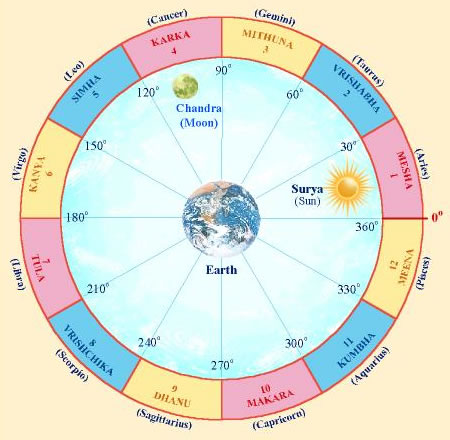
\includegraphics[scale=1]{data/images/jyotish_rashis.jpg}
\end{figure}

The whole universe is seen in the form of a person. The body of the universe consists of the 12 Rashis, which can be roughly translated as “astrological signs.” Each Rashi represents a part of the body. The nine Grahas or planets govern this universal body. The 12 Rashis are represented in the Maharishi Jyotish program as 12 equal segments of a circle, each covering 30 degrees.The sequence of the 12 Rashis begins with Mesha as the first Rashi.

\begin{tabular}{|l | l|}
\hline
\textbf{Vedic Name} & \textbf{English Names} \\ \hline
 Mesha & Aries \\ \hline
 Vrishabha & Taurus\\ \hline
 Mithuna & Gemini\\ \hline
 Karka & Cancer\\ \hline
 Simha & Leo\\ \hline
 Kanya & Virgo\\ \hline
 Tula & Libra\\ \hline
 Vrishchika & Scorpio\\ \hline
 Dhanu & Sagittarius\\ \hline
 Makara & Capricorn\\ \hline
 Kumbha & Aquarius\\ \hline
 Meena & Pisces\\ \hline
\end{tabular}



\end{document}